\documentclass[a4paper]{extarticle}
\usepackage{ctex}
\usepackage{titlesec}
\usepackage{lipsum}
\usepackage{geometry}
\usepackage{amsmath}
\usepackage{biblatex}
\usepackage{booktabs}
\usepackage{caption}
\usepackage{graphicx}
\usepackage{float}
\usepackage{subfig}
\setCJKmainfont{STSong}[AutoFakeBold,AutoFakeSlant]
\setCJKsansfont{Microsoft YaHei}
\setCJKmonofont{KaiTi}
\setmainfont{Times New Roman}
\setsansfont{Times New Roman}
\setmonofont{Times New Roman}
\linespread{1.5}
\setlength{\parindent}{0pt}
\titleformat{\section}{\bfseries\fontsize{14pt}{\baselineskip}\selectfont}{\thesection}{0.5em}{}
\titleformat{\subsection}{\bfseries\fontsize{10.5pt}{\baselineskip}\selectfont}{\thesubsection}{0.5em}{}
\titleformat{\subsubsection}{\fontsize{10.5pt}{\baselineskip}\selectfont}{\thesubsubsection}{0.5em}{}
\geometry{left=2.5cm,right=2.5cm,top=2.5cm,bottom=2.5cm}
\everymath{\displaystyle}

\begin{document}
    \begin{center}
        \textbf{\fontsize{22pt}{\baselineskip} \selectfont 拉伸法测量钢丝杨氏模量}\\
        \vspace{2em}
        \texttt{\fontsize{14pt}{\baselineskip} \selectfont 作者:刘子墨,学号:PB23000233}\\
    \end{center}
    \vspace{2em}
    \hspace{2em}\textsf{\fontsize{9pt}{\baselineskip} \selectfont 摘要:}
    \texttt{\fontsize{9pt}{\baselineskip} \selectfont 本文采用拉伸法测量钢丝的杨氏模量,并利用光杠杆放大法提高测量精度。实验利用增减砝码施加不同的拉力,并测量相应的应变,通过建立应力-应变曲线来确定杨氏模量。利用光杠杆放大原理,我们提高了测量应变的灵敏度和准确性。实验结果显示,钢丝的杨氏模量为$1.842\times10^{11}$ Pa,标准不确定度为$5.5\times10^9$ Pa。}
    \par\hspace{2em}\textsf{\fontsize{9pt}{\baselineskip} \selectfont 关键词:}
    \texttt{\fontsize{9pt}{\baselineskip} \selectfont 杨氏模量;光杠杆放大法;不确定度分析}\\ 
    \section{引言}
    \hspace{2em}
    杨氏弹性模量(简称杨氏模量)是表征刚性材料在弹性限度内材料抗压或拉伸性能的物理量,它仅取决于材料本身的物理性质,与样品的尺寸大小、外形和外加力的大小无关。杨氏模量的大小标志了材料的刚性程度,杨氏模量越大,则越不容易发生形变,它是工程技术中常用的重要力学参数。
    \par\hspace{2em}
    在材料弹性限度内,应力 $F/S$(即法向力与力所作用的面积之比)和应变 $\Delta L/L$ (即长度的变化与原来的长度)之比是一个常数,即:
    \begin{equation}
        E=\frac{F/S}{\Delta L/L}=\frac{FL}{S\Delta L}
        \label{eq:yangshimoliang}
    \end{equation}
    式中 E 称为材料的杨氏模量。
    \par\hspace{2em}
    根据式\ref{eq:yangshimoliang}可以计算出材料的杨氏模量 $E$ 。因为刚性材料在外力拉伸下一般伸长量 $\Delta L$ 很小,所以采用光学放大法,将其放大。本实验采用光杠杆放大法测量 $\Delta L$ 。
    \section{实验内容与设计}
    \subsection{实验装置}
    \hspace{2em}
    杨氏模量测量仪(如图所示),500 g砝码 6 个,钢卷尺,螺旋测微器,水平仪。
    \begin{figure}[H]
        \centering
        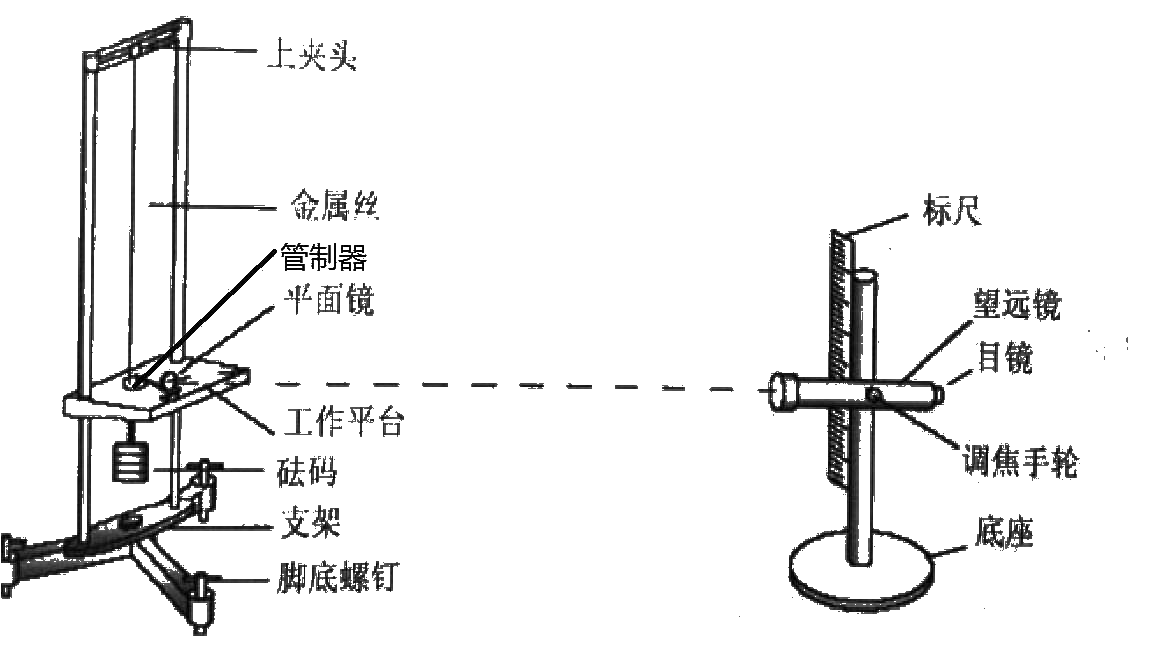
\includegraphics[width=0.8\textwidth]{zhuangzhi.png}
        \caption{测量杨氏模量的实验装置}
    \end{figure}
    待测金属丝长约 1m,其上端夹紧悬挂于支架顶部,穿过中空的圆柱形管制器后,下端被管制器底部夹紧,支架中部有一平台,平台中一圆孔,管制器能在孔中上下自由移动,砝码加在管制器下的砝码托上,金属丝因受到拉力而伸长。砝码加在砝码托上,拉伸钢丝,钢丝伸长后带动管束器下降,光杆杠后足随之下降。从望远镜中观察标尺读数的变化,即可推算出伸长量 $\Delta L$ 。
    \subsection{实验方案}
    \hspace{2em}
    根据公式\ref{eq:yangshimoliang},我们可以通过测量拉力 $F$ 和伸长量 $\Delta L$ 来计算杨氏模量 $E$ 。拉力 $F$ 可以通过砝码的重力来测量,伸长量 $\Delta L$ 可以通过光杠杆放大法来测量。
    \par\hspace{2em}
    如图\ref{fig:guangganggan},光杠杆是一个带有可旋转平面镜的支架,平面镜的镜面基本垂直于刀口和足尖所决定的平面,其后足即杠杆的支脚与被测物接触。
    \begin{figure}[H]
        \centering
        \subfloat[光杠杆结构图]{\label{fig:guangganggan}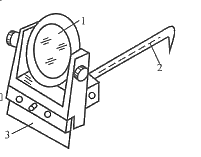
\includegraphics[height=0.2\textwidth]{guangganggan.png}}
        \subfloat[光杠杆工作原理]{\label{fig:yuanli}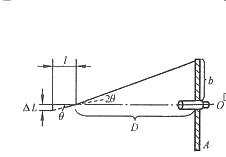
\includegraphics[height=0.2\textwidth]{yuanli.png}}
        \caption{光杠杆结构和工作原理}
    \end{figure}
    \par\hspace{2em}当金属丝受到向下拉力 F 作用时,杠杆支脚将随被测物下降微小距离 $\Delta L$ ,平面镜镜面的法线将转过一个 $\theta$ 角,此时从望远镜中看到的标尺刻度是标尺经过平面镜反射所成的像,从尺子发出的入射线和反射线的夹角为 $2\theta$ ,如图\ref{fig:yuanli}所示,当 $\theta$ 很小时,有:
    \begin{equation*}
        \theta\approx\tan\theta=\frac{\Delta L}{l}
    \end{equation*}
    式中 $l$ 为光杠杆的臂长。由图\ref{fig:yuanli}可知:
    \begin{equation*}
        \tan2\theta\approx2\theta=\frac{b}{D}
    \end{equation*}
    式中 $D$ 为镜面到标尺的距离, $b$ 为在拉力 $F$ 作用下标尺读数的改变。进而可以得到:
    \begin{equation*}
        \Delta L=\frac{bl}{2D}
    \end{equation*}
    \begin{equation}
        E=\frac{2DLF}{Slb}
        \label{eq:1}
    \end{equation}
    式中 $\frac{2D}{L}$ 叫做光杠杆的放大倍数。测出 $D$ 、$L$ 、 $l$ 和金属丝直径 $d$ 及一系列的 $F$ 与 $b$ 之后,由式\ref{eq:1}即可计算出金属丝的杨氏模量 $E$。
    \subsection{实验步骤}
    \subsubsection{调节仪器}
    \begin{enumerate}
        \item 调节支架底部螺丝,确保平台的水平;调节平台的上下位置,使管制器顶部与平台的上表面共面。
        \item 光杠杆的调节。调节光杠杆处于正常工作状态。
        \item 镜尺组的调节。调节望远镜、直尺和光杠杆三者之间的相对位置,调节望远镜目镜及物镜焦距,使标尺像清晰。
    \end{enumerate}
    \subsubsection{测量}
    \begin{enumerate}
        \item 记录望远镜中标尺的初始读数 $b_0$ 作为钢丝的起始长度。
        \item 在砝码托上逐次加相同质量的砝码,记录每增加一个砝码时望远镜中标尺上的读数$b_i$ ,然后再将砝码逐次减去,记下对应的读数 $b_i'$ ,取相同砝码的两组数据的平均值 $\overline{b_i}$ 。
        \item 用钢卷尺分别重复测量三次金属丝的长度 $L$ ,平面镜与标尺之间的距离 $D$ ,光杠杆的臂长 $l$ ,用螺旋测微器重复测量六次金属丝直径 $d$ 。
    \end{enumerate}
    \subsubsection{数据处理}
    \hspace{2em}
    把式\ref{eq:1}改写为:
    \begin{equation*}
        b_i=\frac{2DLF_i}{SlE}=MF_i
    \end{equation*}
    其中 $M=\frac{2DL}{FlE}$ ,在一定的实验条件下, $M$ 是一个常量。用最小二乘法拟合 $b_i$ 和 $F_i$ ,其斜率为 $M$。进而可由式\ref{eq:celiang}计算杨氏模量:
    \begin{equation}
        E=\frac{2DL}{SlM}
        \label{eq:celiang}
    \end{equation}
    \section{实验结果和讨论}
    \subsection{测量值及其不确定度}
    \hspace{2em}
    金属丝的长度 $L$ ,平面镜与标尺之间的距离 $D$ ,光杠杆的臂长 $l$ 的测量数据如下:
    \begin{table}[H]
        \centering
        \caption{$L$、$D$、$l$ 的测量数据}
        \begin{tabular}{cccc}
            \toprule
             & 金属丝长度 $L$ /cm & 平面镜与标尺之间的距离 $D$ /cm & 光杠杆的臂长 $l$/cm\\
            \midrule
            第一次测量 & 96.0 & 153.6 & 7.4\\
            第二次测量 & 96.3 & 153.7 & 7.4\\
            第三次测量 & 96.2 & 153.6 & 7.3\\
            \midrule
            平均值 & 96.17 & 153.63 & 7.37\\
            \bottomrule
        \end{tabular}
    \end{table}
    \hspace{2em}
    金属丝直径 $d$ 的测量数据如下:
    \begin{table}[H]
        \centering
        \caption{金属丝直径 $d$ 的测量数据}
        \begin{tabular}{cc}
            \toprule
             & 金属丝直径 $d$ /mm\\
            \midrule
            第一次测量 & 0.30\\
            第二次测量 & 0.30\\
            第三次测量 & 0.30\\
            第四次测量 & 0.30\\
            第五次测量 & 0.30\\
            第六次测量 & 0.30\\
            \midrule
            平均值 & 0.300\\
            \bottomrule
        \end{tabular}
    \end{table}
    \subsubsection{金属丝的长度 $L$ 的标准不确定度}
    \hspace{2em}
    实验使用钢卷尺测量金属丝的长度 $L$ ,则的测量模型为:
    \begin{equation*}
        L=\overline{L}+L_0+L_1
    \end{equation*}
    其中$\overline{L}$为钢卷尺直接读出的长度,$L_0$为钢卷尺的仪器误差对测量的影响,$L_1$为使用卷尺测量摆长时难以完全对齐对测量结果的影响,作为保守估计,一般可取最大不确定度$\Delta_B\approx$ 0.2 cm。考虑到测量精度要求,测量模型中忽略了其他因素的影响。
    \par\hspace{2em}
    钢卷尺直接读出的金属丝的长度$\overline{L}$为A类,其不确定度$\mu_{\overline{L}}$为:
    \begin{equation*}
        \mu_{\overline{L}}=\sqrt{\frac{\sum\limits_{i=1}^{n}(L_i-\overline{L})^2}{n(n-1)}}=8.8\times10^{-4}\,\text{m}
    \end{equation*}
    钢卷尺的仪器误差$L_0$为B类正态分布,实验中用 2 m 量程钢卷尺的最大允差为 0.0012
    m,其不确定度$\mu_{L_0}$为:
    \begin{equation*}
        \mu_{L_0}=\frac{\Delta_\text{尺}}{3}=4\times10^{-4}\,\text{m}
    \end{equation*}
    \hspace{2em}
    使用卷尺测量金属丝长度时难以完全对齐对测量结果的影响$L_1$呈B类正态分布,取最大不确定度$\Delta_B\approx$ 0.2 cm,则其不确定度为:
    \begin{equation*}
        \mu_{L_1}=\frac{\Delta_B}{3}=6.67\times10^{-4}\,\text{m}
    \end{equation*}
    \hspace{2em}
    所以金属丝的长度$L$的不确定度为:
    \begin{equation*}
        \mu_L=\sqrt{\mu_{\overline{L}}^2+\mu_{L_0}^2+\mu_{L_1}^2}=1.2\times10^{-3}\,\text{m}
    \end{equation*}
    \subsubsection{平面镜与标尺之间的距离 $D$ 的标准不确定度}
    \hspace{2em}
    实验使用钢卷尺测量平面镜与标尺之间的距离 $D$ ,则的测量模型为:
    \begin{equation*}
        D=\overline{D}+D_0+D_1
    \end{equation*}
    其中$\overline{D}$为钢卷尺直接读出的长度,$D_0$为钢卷尺的仪器误差对测量的影响,$D_1$为使用卷尺测量摆长时难以完全对齐对测量结果的影响,作为保守估计,一般可取最大不确定度$\Delta_B\approx$ 0.2 cm。考虑到测量精度要求,测量模型中忽略了其他因素的影响。
    \par\hspace{2em}
    钢卷尺直接读出的平面镜与标尺之间的距离$\overline{D}$为A类,其不确定度$\mu_{\overline{D}}$为:
    \begin{equation*}
        \mu_{\overline{D}}=\sqrt{\frac{\sum\limits_{i=1}^{n}(D_i-\overline{D})^2}{n(n-1)}}=3.3\times10^{-4}\,\text{m}
    \end{equation*}
    \hspace{2em}
    钢卷尺的仪器误差$D_0$和测量时难以完全对其造成的误差$D_1$与上面相同,所以平面镜与标尺之间的距离$D$的不确定度为:
    \begin{equation*}
        \mu_D=\sqrt{\mu_{\overline{D}}^2+\mu_{D_0}^2+\mu_{D_1}^2}=8.4\times10^{-4}\,\text{m}
    \end{equation*}
    \subsubsection{光杠杆的臂长 $l$ 的标准不确定度}
    \hspace{2em}
    实验使用钢卷尺测量光杠杆的臂长 $l$ ,则的测量模型为:
    \begin{equation*}
        l=\overline{l}+l_0+l_1
    \end{equation*}
    其中$\overline{l}$为钢卷尺直接读出的长度,$l_0$为钢卷尺的仪器误差对测量的影响,$l_1$为使用卷尺测量摆长时难以完全对齐对测量结果的影响,作为保守估计,一般可取最大不确定度$\Delta_B\approx$ 0.2 cm。考虑到测量精度要求,测量模型中忽略了其他因素的影响。
    \par\hspace{2em}
    钢卷尺直接读出的光杠杆的臂长$\overline{l}$为A类,其不确定度$\mu_{\overline{l}}$为:
    \begin{equation*}
        \mu_{\overline{l}}=\sqrt{\frac{\sum\limits_{i=1}^{n}(l_i-\overline{l})^2}{n(n-1)}}=3.3\times10^{-4}\,\text{m}
    \end{equation*}
    \hspace{2em}
    钢卷尺的仪器误差$l_0$和测量时难以完全对其造成的误差$l_1$与上面相同,所以光杠杆的臂长$l$的不确定度为:
    \begin{equation*}
        \mu_l=\sqrt{\mu_{\overline{l}}^2+\mu_{l_0}^2+\mu_{l_1}^2}=8.4\times10^{-4}\,\text{m}
    \end{equation*}
    \subsubsection{金属丝直径 $d$ 的标准不确定度}
    \hspace{2em}
    金属丝直径 $d$ 的测量模型为:
    \begin{equation*}
        d=\overline{d}+d_0
    \end{equation*}
    其中$\overline{d}$为测量的平均值,$d_0$为螺旋测微器的仪器误差。考虑到测量精度要求,测量模型中忽略了其他因素的影响。
    \par\hspace{2em}
    螺旋测微器直接读出的金属丝直径$d$为A类,其不确定度$\mu_{\overline{d}}$为:
    \begin{equation*}
        \mu_{\overline{d}}=\sqrt{\frac{\sum\limits_{i=1}^{n}(d_i-\overline{d})^2}{n(n-1)}}=0
    \end{equation*}
    \par\hspace{2em}
    螺旋测微器的仪器误差$d_0$为B类均匀分布,实验中用 0.01 mm 量程螺旋测微器的最大允差为 0.004 mm,其不确定度$\mu_{d_0}$为:
    \begin{equation*}
        \mu_{d_0}=\frac{\Delta_\text{螺旋}}{\sqrt{3}}=2.3\times10^{-6}\,\text{m}
    \end{equation*}
    \hspace{2em}
    所以金属丝直径$d$的不确定度为:
    \begin{equation*}
        \mu_d=\sqrt{\mu_{\overline{d}}^2+\mu_{d_0}^2}=2.3\times10^{-6}\,\text{m}
    \end{equation*}
    \subsection{线性拟合结果及其不确定度}
    \hspace{2em}
    金属丝的拉力 $F$ 和标尺读数 $b$ 的测量数据如下(取$g=9.795$ m/s$^2$):
    \begin{table}[H]
        \centering
        \caption{拉力 $F$ 和标尺读数 $b$ 的测量数据}
        \begin{tabular}{ccccc}
            \toprule
            砝码个数 & 拉力 $F$ /N & 标尺读数1 $b_1$ /cm & 标尺读数2 $b_2$ /cm & 标尺平均读数 $\overline{b}$ /cm\\
            \midrule
            0 & 0 & -0.5 & -0.5 & -0.50\\
            1 & 4.8975 & 1.5 & 1.4 & 1.45\\
            2 & 9.7950 & 3.3 & 3.3 & 3.30\\
            3 & 14.7825 & 5.0 & 5.2 &5.10\\
            4 & 19.6800 & 6.6 & 6.7 & 6.65\\
            5 & 24.5775 & 8.2 & 8.3 & 8.25\\
            6 & 29.4750 & 9.8 & 9.8 & 9.80\\
            \bottomrule
        \end{tabular}
    \end{table}
    \hspace{2em}
    在origen绘图软件中使用最小二乘法进行拟合:
    \begin{figure}[H]
        \centering
        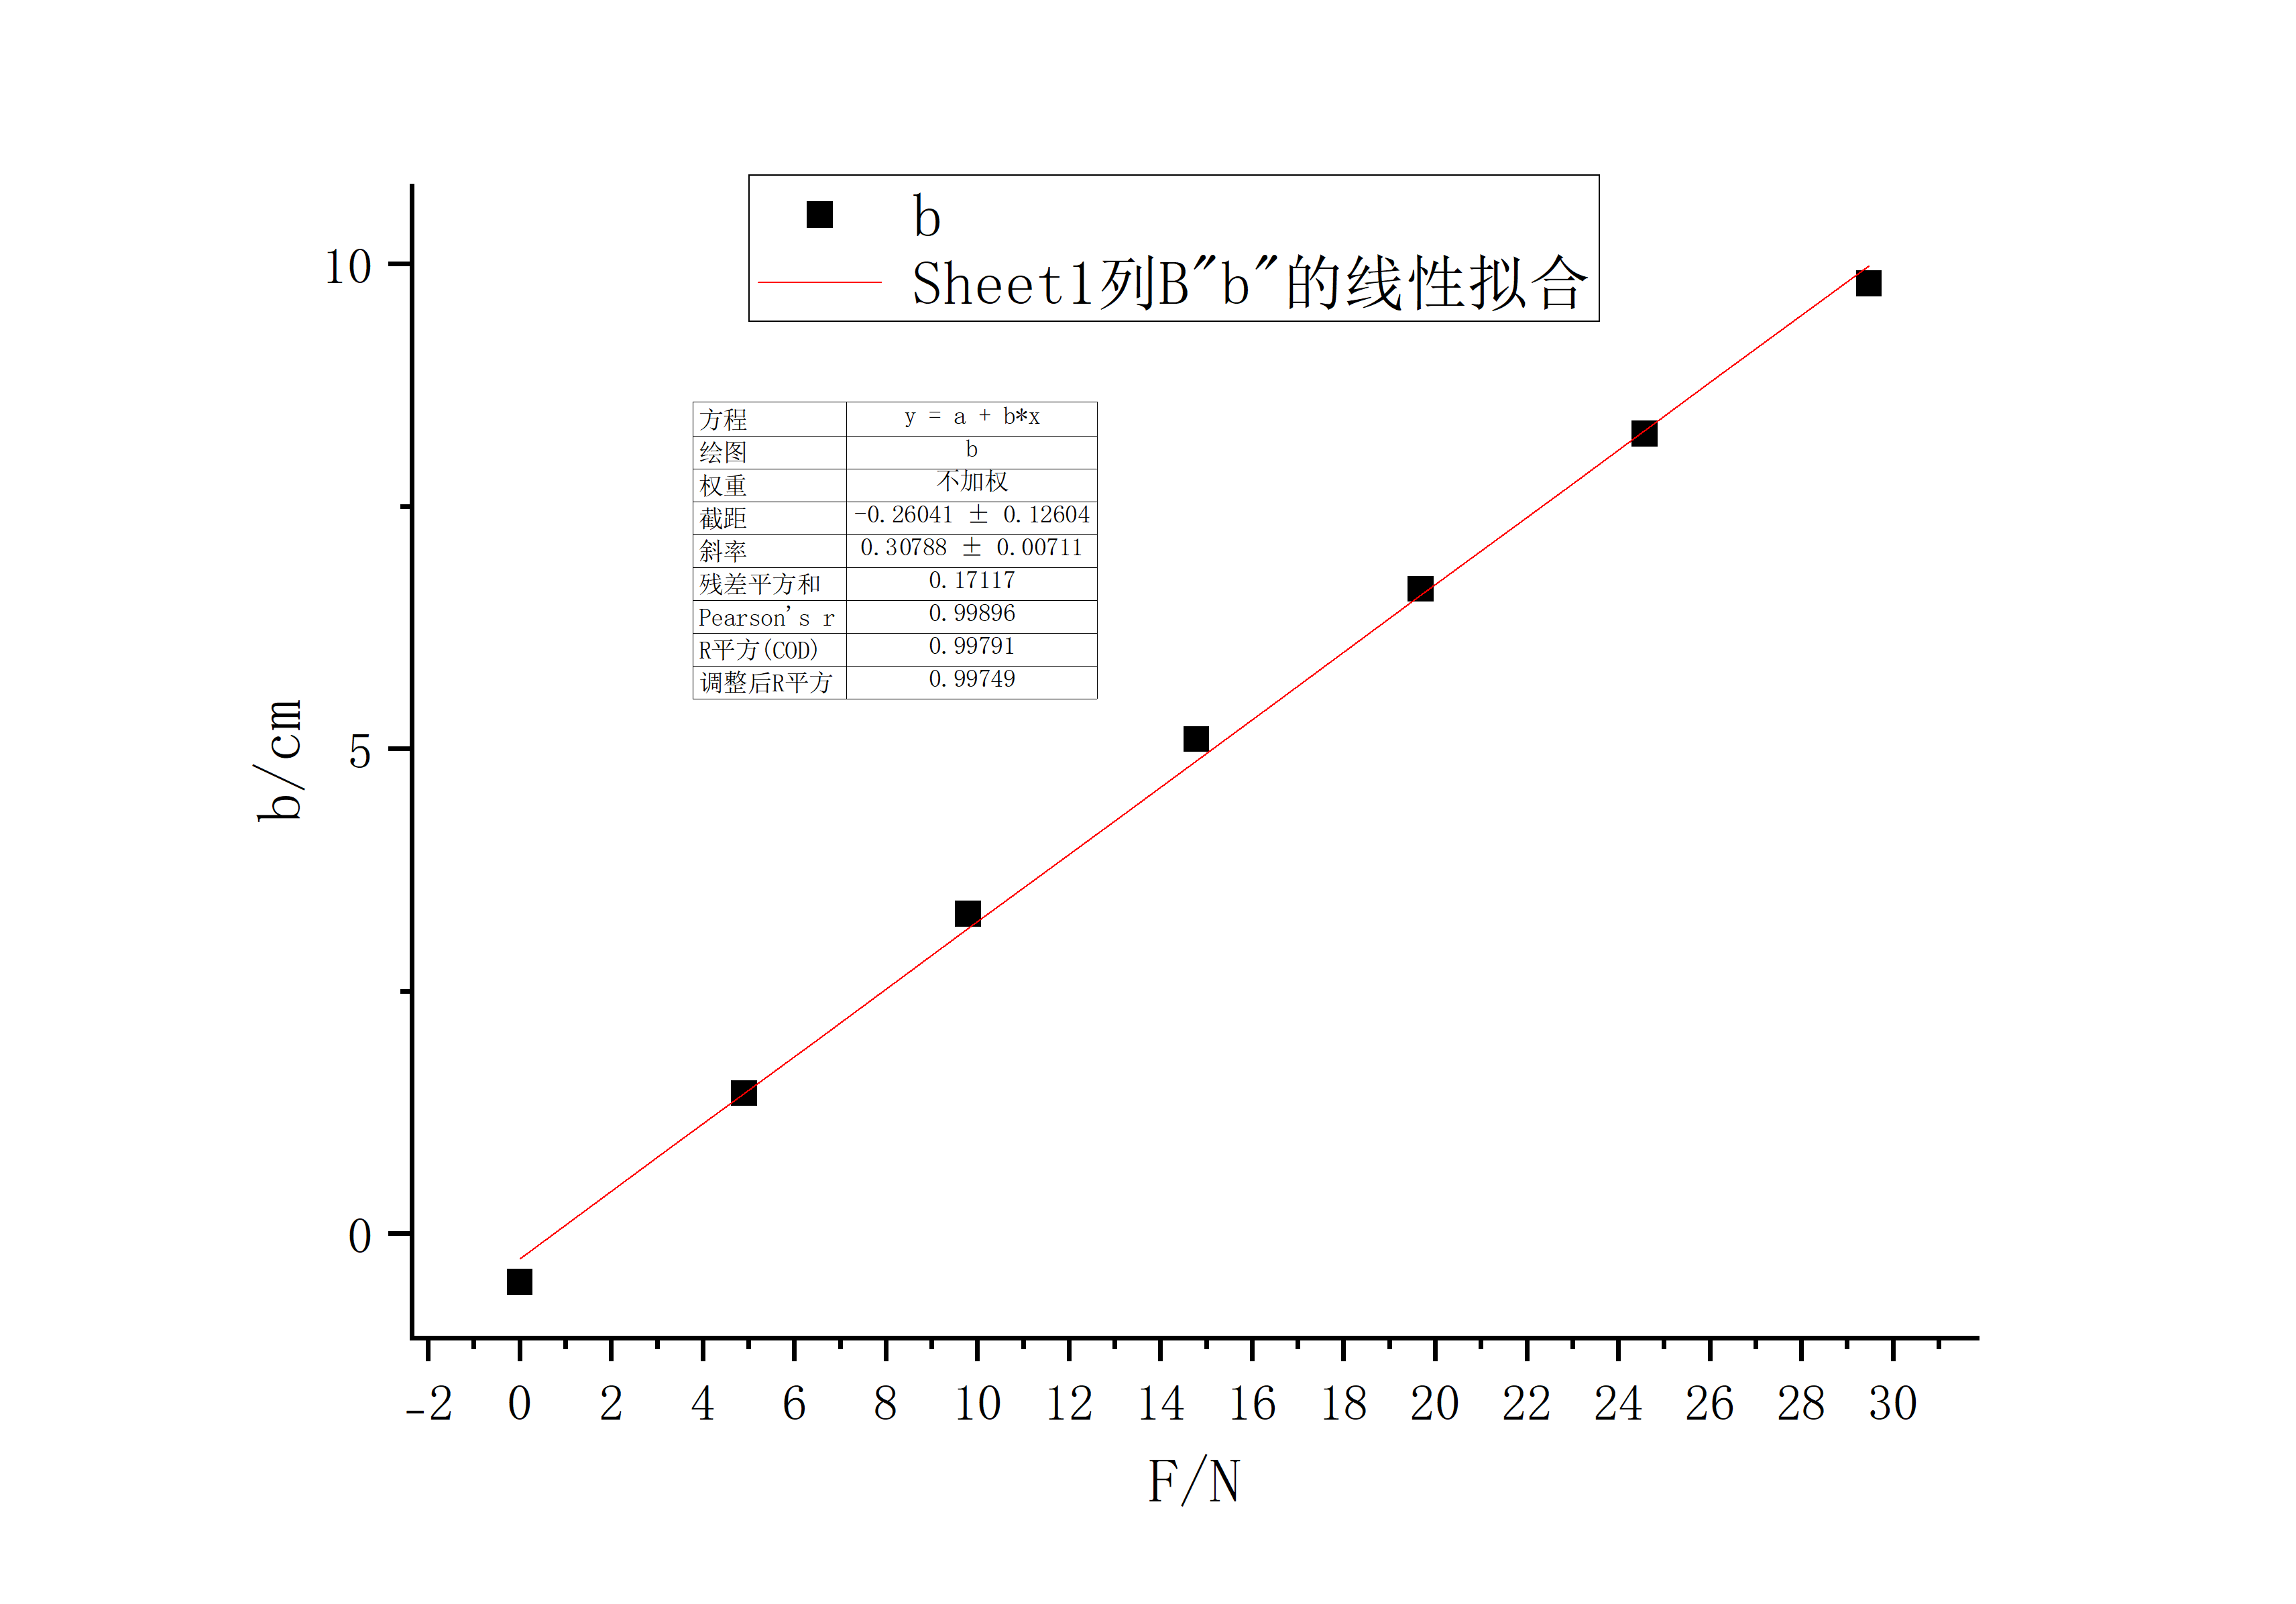
\includegraphics[width=0.8\textwidth]{nihe.png}
        \caption{拉力 $F$ 和标尺读数 $b$ 的拟合图}
    \end{figure}
    拟合得到斜率为$M=3.079\times10^{-3}$ m/N,其不确定度为 $\mu_M=7.1\times10^{-5}$ m/N截距为$C=-0.2604$ cm,相关系数为$r=0.9989$。
    \subsection{杨氏模量的计算结果及其不确定度}
    \hspace{2em}
    代入测量公式式\ref{eq:celiang},可得杨氏模量测量值为:
    \begin{equation*}
        E=\frac{2DL}{SlM}=\frac{2\times1.5363\times0.9617}{\frac{1}{4}\pi\left(3\times10^{-4}\right)^2\times0.0737\times3.079\times10^{-3}}=1.842\times10^{11}\,\text{Pa}
    \end{equation*}
    \hspace{2em}
    根据测量公式式\ref{eq:celiang}杨氏模量的不确定度计算公式为:
    \begin{equation*}
        \mu_E=E\sqrt{\left(\frac{\mu_D}{D}\right)^2+\left(\frac{\mu_L}{L}\right)^2+\left(\frac{\mu_l}{l}\right)^2+\left(\frac{2\mu_d}{d}\right)^2+\left(\frac{\mu_M}{M}\right)^2}=5.5\times10^9\,\text{Pa}
    \end{equation*}
    \hspace{2em}
    所以杨氏模量的测量结果为$E=(1.842\pm0.055)\times10^{11}$ Pa。
    \section{结论}
    \hspace{2em}
    本实验采用拉伸法测量钢丝的杨氏模量,并利用光杠杆放大法提高测量精度。实验结果显示,钢丝的杨氏模量为$1.842\times10^{11}$ Pa,标准不确定度为$5.5\times10^9$ Pa,约为$3\%$,说明实验结果较为准确。误差来源主要来源于:
    \begin{enumerate}
        \item 钢丝长度和平面镜与标尺间距离较大,在测量过程中会出现卷尺弯折的情况,故容易造成测量不准确;
        \item 光杠杆为精密仪器,任何细微的扰动都会带来误差,而在测量的过程中其很容易受到扰动,所以存在偶然误差;
        \item 实验器材的时间较长,钢丝易发生变形,导致钢丝各位置的粗细不一,从而会产生较大的不确定度。
    \end{enumerate}
    \section{思考题}
    \subsection{预习思考题}
    \begin{enumerate}
        \item 什么是材料的杨氏模量,它和材料的长度、横截面积是否有关?
        \par
        杨氏模量是表征刚性材料在弹性限度内材料抗压或拉伸性能的物理量,定义式为应力与应变之比$E=\frac{F/S}{\Delta L/L}$,它仅取决于材料本身的物理性质,与材料的长度、横截面积无关。
        \item 光杠杆放大原理是什么,它的放大倍数由那些量决定?
        \par
        光杠杆是一个带有可旋转平面镜的支架,平面镜的镜面基本垂直于刀口和足尖所决定的平面,其后足即杠杆的支脚与被测物接触。当被测物受到向下拉力 F 作用时,杠杆支脚将随被测物下降微小距离 $\Delta L$ ,平面镜镜面的法线将转过一个 $\theta$ 角,此时从望远镜中看到的标尺刻度是标尺经过平面镜反射所成的像,从尺子发出的入射线和反射线的夹角为 $2\theta$ 。光杠杆的放大倍数由光杠杆的臂长 $l$ 和镜面到标尺的距离 $D$ 决定。
    \end{enumerate}
    \subsection{实验过程思考题}
    \begin{enumerate}
        \item 实验过程中,如果从望远镜中看到的尺子不清晰是因为什么,如何调节
        才能使得尺子读数清晰?
        \par
        望远镜中看到的尺子不清晰可能是因为尺子的像不在望远镜的焦平面上,可以通过调节望远镜焦距,使标尺像清晰。
        \item 实验过程中,当从望远镜看到尺子的初始值较大,调节什么仪器可以使
        得初始值较小,以免加砝码后读数溢出?
        \par
        先检查望远镜、光杠杆的平面镜和标尺零刻度线位置是否大约在同一高度。如果不在同一高度,调节三者约在同一高度;如果在同一高度,应检查光杠杆平面镜是否位于竖直方向,调节光杠杆平面镜使其竖直并使标尺零刻度线位于视野中央。
        \item 如何准确测量光杠杆的臂长?
        \par
        使用钢卷尺测量光杠杆的臂长,测量时注意尽量使钢卷尺平直,避免弯曲,并重复测量三次,使得测量结果尽可能准确。
    \end{enumerate}
    \subsection{实验报告思考题}
    \begin{enumerate}
        \item 利用光杠杆把测微小长度$\Delta L$ 变成测 $b$,光杠杆的放大率为 $\frac{2D}{L}$,根据此式能否以增加 $D$ 减小 $l$来提高放大率,这样做有无好处?有无限度?应怎样考虑这个问题?
        \par
        可以以增加 $D$ 减小 $l$ 来提高放大率。但是增加$D$会使得使用钢卷尺测量时弯曲的可能性增大,从而影响测量的准确性。减小 $l$ 会使得光杠杆的稳定性降低,从而影响测量的准确性;并且$L$减小过多会导致不满足小角近似的条件,使公式失效。而且放大倍数太大会导致增加砝码后标尺示数超过量程,并且会放大标尺、光杠杆的平面镜倾斜带来的误差。所以在实际操作中,应该综合考虑,在合适的范围内增加$D$和减小$l$来提高放大率。
        \item 实验中,各个长度量用不同的仪器来测量是怎样考虑的,为什么?
        \par
        金属丝的长度 $L$ 、平面镜与标尺之间的距离 $D$ 、光杠杆的臂长 $l$ 用钢卷尺测量。因为金属丝的长度 $L$ 、平面镜与标尺之间的距离 $D$ 较长,常见的测量仪器中只有钢卷尺的量程可以测量这些长度。从量程上考虑,光杠杆的臂长 $l$ 可以使用钢卷尺或游标卡尺测量,但是从不确定度上考虑,游标卡尺虽然仪器允差更小,但是不会对最终测量杨氏模量 $E$ 的不确定度产生显著影响,所以没有必要使用精度更高的游标卡尺,选用钢卷尺测量光杠杆臂长 $l$ 。
        \par
        金属丝直径 $d$ 用螺旋测微器测量。螺旋测微器的测量范围较小,测量精度较高,测量的不确定度更小。如果用精度稍低的游标卡尺测量,会使得最终测量杨氏模量 $E$ 的不确定度显著增大。
    \end{enumerate}
    \section*{参考文献}
    [1]用拉伸法测量钢丝的杨氏模量. 实验讲义,2024\par
    [2]吴泳华,霍剑青,浦其荣. 大学物理实验. 北京:高等教育出版社,2005.11,137-141\par
    [3]张志东,魏怀鹏,展永. 大学物理实验(第四版),2011.8,北京:科学出版社,129-134\par
    [4]徐建强,徐荣历. 大学物理实验(第二版). 北京:科学教育出版社,2014.1,220-225\par
    [5]孙丽媛,祖新慧. 大学物理实验. 北京:清华大学出版社,2014.4,42-46\par
    [6]江美福,方建性 大学物理实验教程. 北京:科学出版社,2009.08 104-106\par
    [7]张海鲲,邵明辉,崔晓军. 大学物理实验. 北京:高等教育出版社,2015.8,153-157\par
    [8]毛爱华,武娥. 大学物理实验. 北京:机械工业出版社,2015.1,53-56
    \newpage
    \section*{附录}
    \subsection*{老师签字的实验数据}
    \begin{figure}[H]
        \centering
        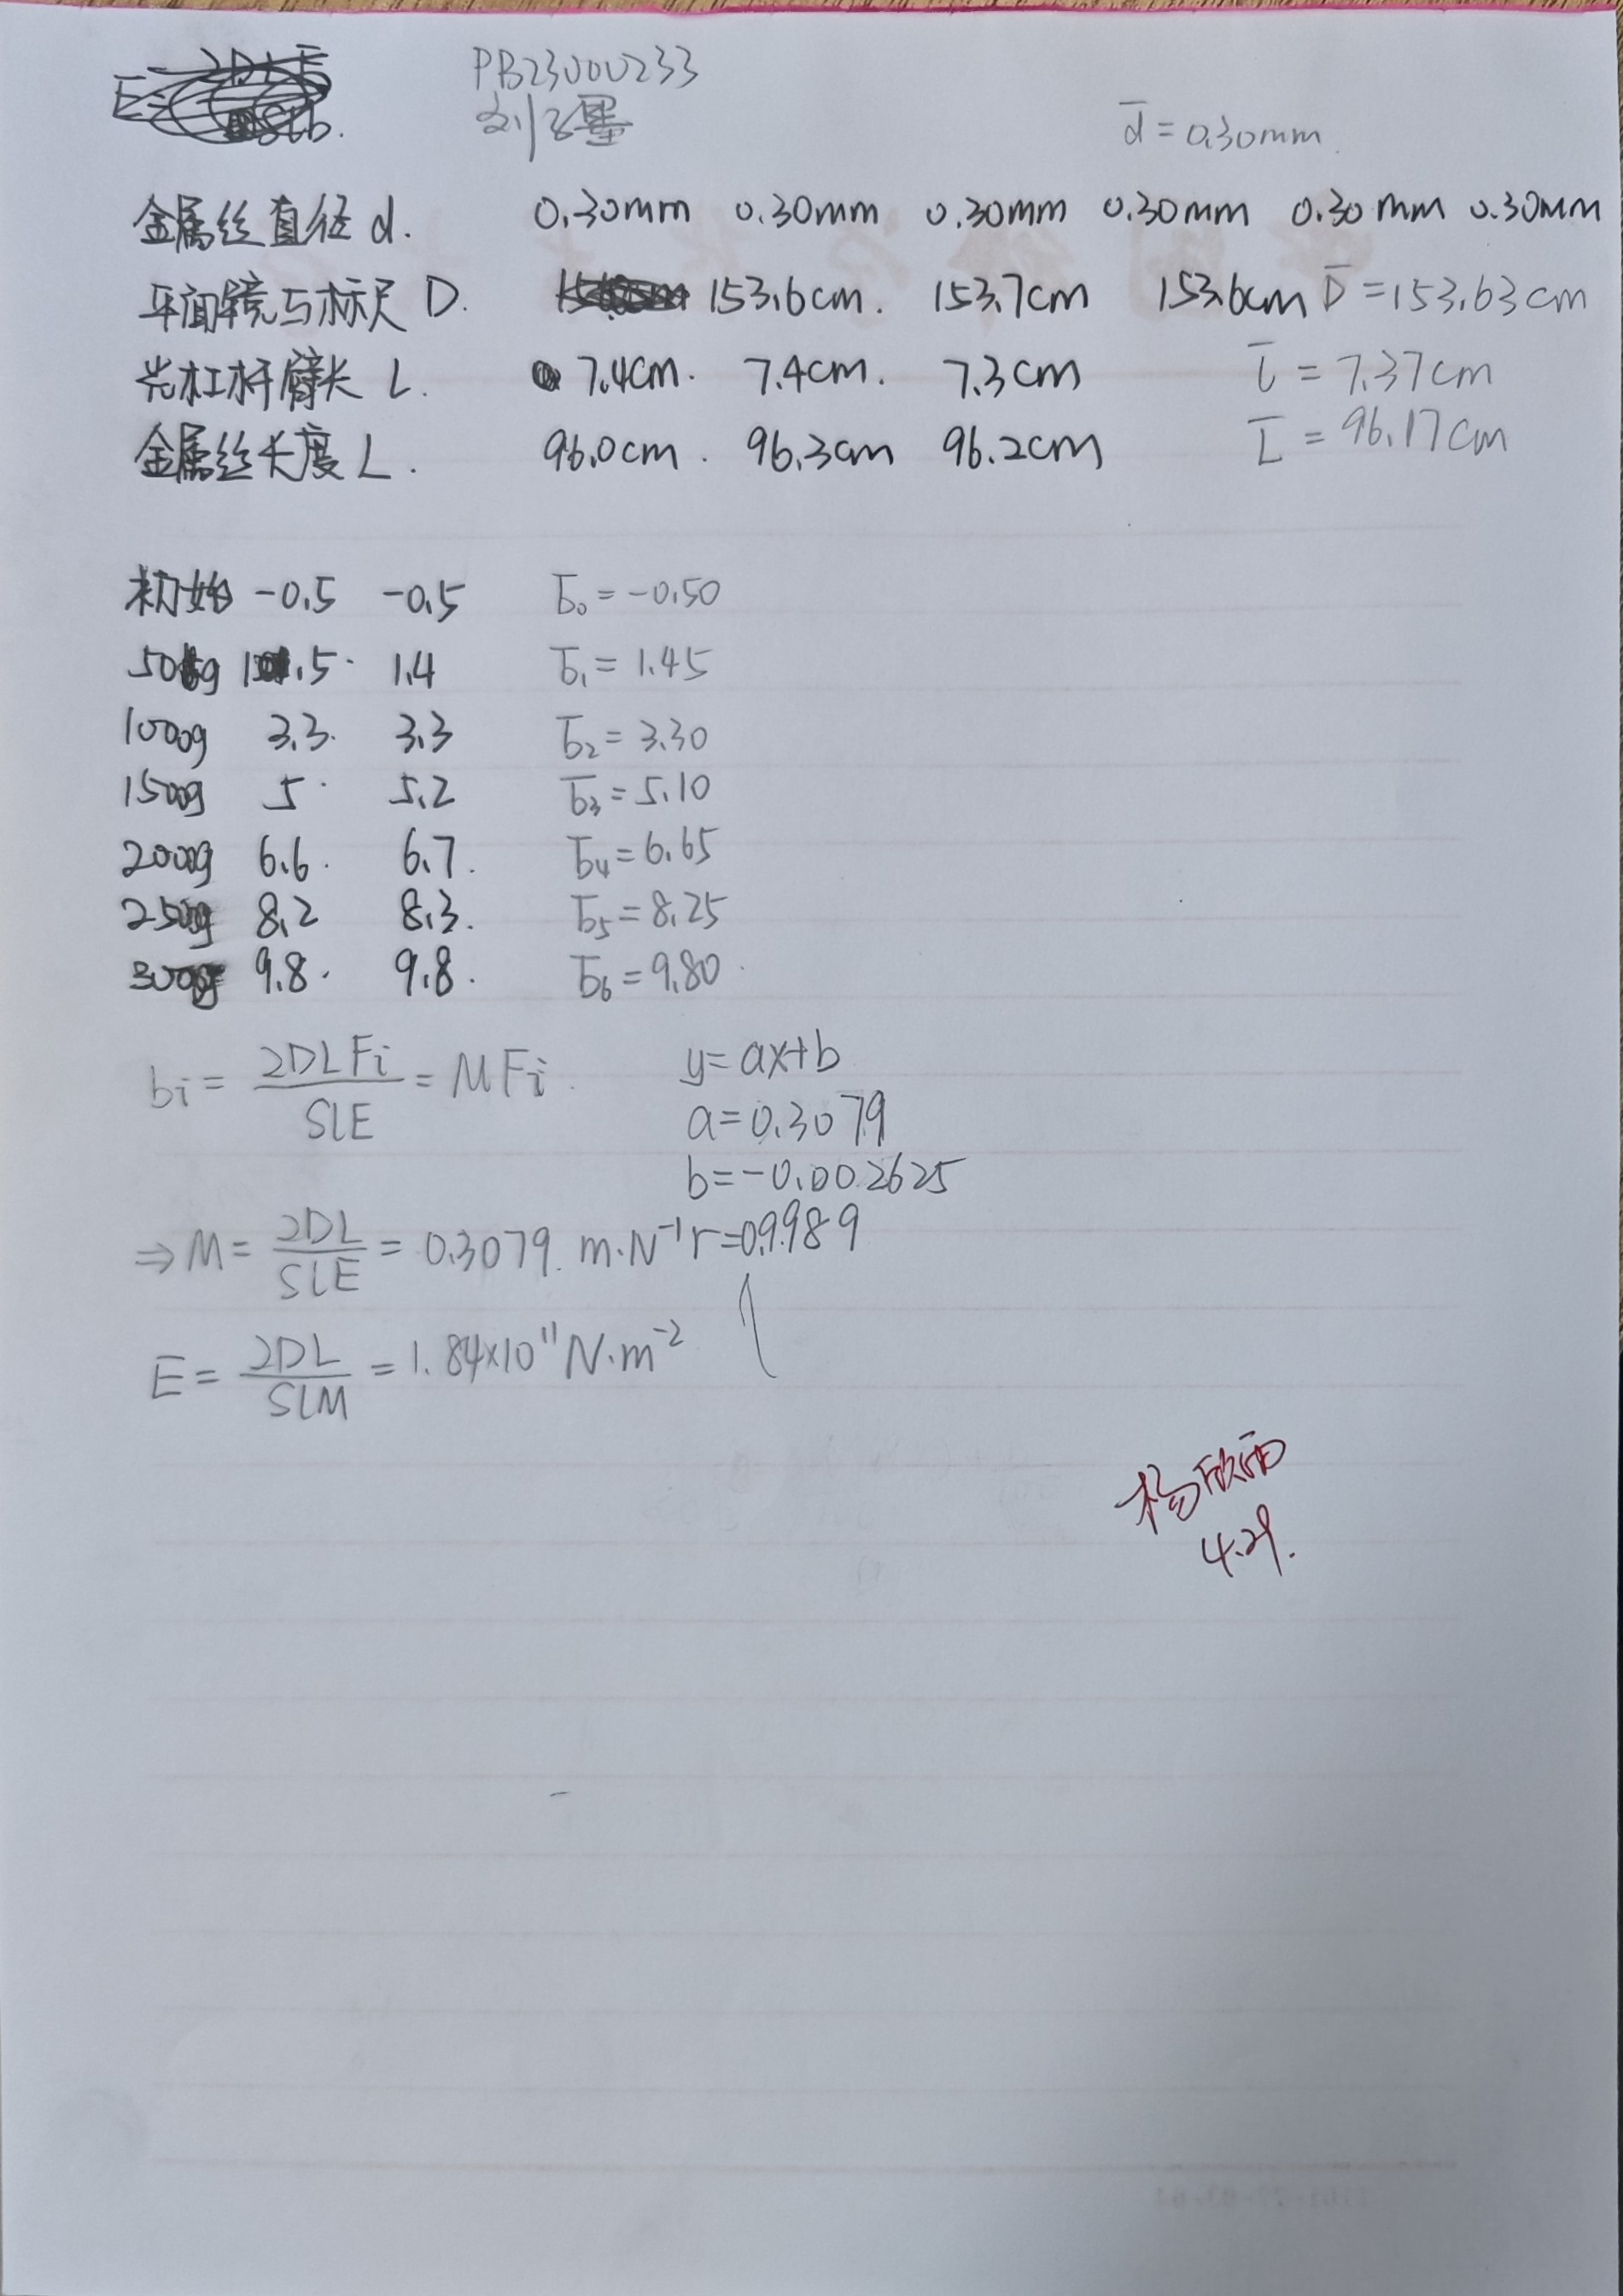
\includegraphics[width=\linewidth]{shuju.jpg}
    \end{figure}
\end{document}
